%% Extended version of the TAS 2026 short paper (AAAI Fall Symposium Series).
%% Venue-neutral preprint. Compiles with pdfLaTeX (Overleaf) or XeLaTeX/Tectonic.
%% Every number is regenerated by scripts/censoring/ and scripts/extended/.

\documentclass[11pt]{article}

\usepackage{iftex}
\ifPDFTeX
  \usepackage[T1]{fontenc}
  \usepackage{newtxtext,newtxmath}
\else
  \usepackage{amssymb}
  \usepackage{fontspec}
  \setmainfont{texgyretermes}[Extension=.otf,UprightFont=*-regular,BoldFont=*-bold,
    ItalicFont=*-italic,BoldItalicFont=*-bolditalic]
\fi
\usepackage[margin=1in]{geometry}
\usepackage{amsmath,amsthm}
\usepackage{graphicx}
\usepackage{booktabs}
\usepackage[numbers,sort&compress]{natbib}
\usepackage[hidelinks]{hyperref}
\usepackage{microtype}
\usepackage{enumitem}
\setlist{itemsep=2pt,topsep=3pt}
\setlength{\emergencystretch}{3em}

\newtheorem{proposition}{Proposition}
\theoremstyle{definition}
\newtheorem{definition}{Definition}
\theoremstyle{remark}
\newtheorem{remark}{Remark}

\newcommand{\pb}{\bar\pi}
\newcommand{\E}{\mathbb{E}}

\title{Invalid Is Not Failure:\\[2pt]
\large Identification, Estimation, and Leaderboard Fragility When\\
Infrastructure Fails in Long-Horizon Agent Evaluation}
\author{Shilin Chhabra\\
University of Wisconsin--Madison\\
\texttt{chhabra7@wisc.edu}}
\date{}

\begin{document}
\maketitle

\begin{abstract}
Long-running agents often stop without a valid task outcome because a provider,
runtime, or evaluation harness failed rather than the agent. Benchmarks then
either score such runs as failures or drop them. We treat this as an
identification problem and make four contributions. First, we give a rule that
separates censoring from failure and show that, when infrastructure failures
are independent of the agent, both common policies are closed-form functions of
three numbers: the success rate and the mean survival probabilities of
successful and failed runs. Scoring invalid runs as failures multiplies the
success probability by the survival of successes; dropping them multiplies the
success odds by the survival ratio; rerunning removes only the between-task part
of that distortion. Second, we show that weighting requires only observed
quantities, give a doubly robust estimator that also uses the partial
trajectory of each invalid run, and give a sensitivity analysis for
outcome-dependent failure. Third, we measure the problem on public data: a
census of 243 SWE-bench leaderboard submissions and 19{,}500 frontier-model runs
on the bash-only leaderboard. Invalid or unattributable runs appear in 70\% of
SWE-bench Verified submissions, and under a broad reading the data identify only
43 of 105 adjacent leaderboard orderings. One frontier submission lost 56\% of
its runs to provider errors, all but one scored as failures; another moves from 12th to
9th of 39 once 11 provider failures are treated as censored, and stays in 9th or
10th unless failed runs are assumed four times less likely to succeed than
comparable completed runs. Fourth, under declared hazards, rankings of 39
frontier models are far more fragile than older corpora: a per-step hazard of
0.1\%, which invalidates about 4\% of runs, already reverses 24 of 741 model
pairs under the standard policy. We release the census, code, and a minimum
validity record for benchmark reports.
\end{abstract}

\section{Introduction}

A long-horizon agent run can end for two very different reasons. The agent can
fail the task, or the measurement apparatus can fail the agent: a provider
returns 503 until the retry budget is exhausted, a container crashes, the
evaluation harness never produces a verdict. Only the first is evidence about
the agent. Yet benchmark reports usually collapse both into one success rate
through an unstated policy: invalid runs are either scored as failures or
deleted. Leaderboards typically do the former, by dividing resolved tasks by
all tasks.

Validity problems in agent benchmarks are well documented
\citep{kapoor2024agentsthatmatter,weidinger2025evalscience,zhu2026guardrails},
and a recent audit finds that agent benchmark papers disclose little about their
harness and failure handling \citep{moghadasi2026disclose}. Our question is
narrower and statistical: \emph{what does each handling policy estimate, what
can the data identify, and how large are the consequences on real
leaderboards?}

The answer is structural. Suppose infrastructure failures are entirely
independent of the agent, arriving with a small hazard per agent step. Long runs
are exposed more often, so an outcome-independent failure becomes informative at
the trajectory level whenever horizon and success are associated. This is the
situation on every corpus we examine, and it is sharpest on the current
frontier, where models differ several-fold in how many steps they take.

\paragraph{Contributions.}
\begin{itemize}
\item \textbf{Identification} (Section~\ref{sec:ident}). A validity rule
separating outcomes from censoring; assumption-free bounds; a three-number
characterisation of the two standard policies; a decomposition of rerunning;
and the observation that weighting needs no counterfactual horizon, with its
limit under hard caps.
\item \textbf{Estimation} (Section~\ref{sec:est}). A doubly robust estimator
that exploits the partial trajectory of every invalid run, and a sensitivity
analysis for outcome-dependent failure.
\item \textbf{Measurement} (Sections~\ref{sec:data}--\ref{sec:real}). A census of
243 public SWE-bench submissions and 19{,}500 frontier runs with harness exit
statuses, showing real invalidity, non-identified leaderboard orderings, and
real rank changes; plus declared-hazard sensitivity on three corpora
($\approx$104k trajectories).
\item \textbf{Practice} (Section~\ref{sec:practice}). A minimum validity record
that makes every estimator in this paper computable from logs.
\end{itemize}

This paper extends a four-page symposium version\footnote{Presented at the AAAI
2026 Fall Symposium on Trustworthy Agentic Systems (TAS 2026). New here: the
estimation theory of Section~\ref{sec:est}, the leaderboard census and frontier
corpus, all real-censoring analyses, and the fragility results on the
frontier.} whose formal core is Section~\ref{sec:ident}.

\section{Setup}
\label{sec:setup}

A benchmark initiates runs $i=1,\dots,N$ with fixed semantic outcomes
$Y_i\in\{0,1\}$ and horizons $H_i$, the number of agent decision steps the run
would take. The estimand is the corpus reliability $p=N^{-1}\sum_iY_i$.
Randomness enters only through the validity indicators $C_i$ (1 if $Y_i$ is
observed), drawn by the infrastructure with $\pi_i=\Pr(C_i=1)$. This
design-based view matches the finite corpora we analyse; population statements
would need i.i.d.\ sampling of runs.

\begin{definition}[Validity rule]\label{def:validity}
Fix the benchmark specification, which declares the agent's budgets (steps,
tokens, cost, context window, wall-clock) and environment. An interruption at
step $k$ is an \emph{outcome} (a valid failure) if a fault-free execution with
the same agent actions up to $k$ would also have terminated there: budget or
context exhaustion, repeated malformed output, or damage the agent did to its
own environment. It is \emph{censoring} if the fault-free execution would not
have terminated: provider errors after retries, host preemption, harness defects,
an evaluation harness that produced no verdict, and wall-clock timeouts whose
budget was consumed by infrastructure latency. Interruptions that cannot be
attributed either way are a third, reported category handled by bounds.
\end{definition}

The context window is part of the system under test, so context exhaustion is a
valid failure and $p$ is success within the declared budgets. The rule is
decidable from logs when budgets are declared in agent-controlled units.

Let $T_i$ be the step at which infrastructure would first fail run $i$, with
survival $G(h)=\Pr(T>h)$. Run $i$ is valid iff $T_i>H_i$, so $\pi_i=G(H_i)$
when $T\perp(Y,H)$. A constant hazard $q$ gives $\pi_i=s^{H_i}$ with $s=1-q$.
Each run reveals $V_i=\min(H_i,T_i)$, $C_i$, and its trajectory prefix up to
$V_i$. Write $\pb_1$ and $\pb_0$ for the mean of $\pi_i$ over successful and
failed runs, $\pb=p\pb_1+(1-p)\pb_0$, $m=1-\pb$ for the expected invalid
fraction, and $\rho=\pb_1/\pb_0$ for the \emph{survival ratio}.

\section{Identification}
\label{sec:ident}

\begin{proposition}[Assumption-free bounds]\label{prop:bounds}
With $M$ censored runs and $S$ observed successes, and no assumption about the
censored outcomes, $S/N\le p\le(S+M)/N$. For bounded scores $Y_i\in[a,b]$ the
endpoints are $(\sum_iC_iY_i+aM)/N$ and $(\sum_iC_iY_i+bM)/N$.
\end{proposition}

This is the agent-evaluation instance of a worst-case bound
\citep{manski1990nonparametric}. Its first consequence is that the standard
leaderboard score, $S/N$, is the \emph{lower endpoint of the identified
interval}, not an estimate of reliability.

\begin{proposition}[Three numbers determine both policies]\label{prop:three}
For any observation probabilities $\pi_i$, including outcome-dependent ones,
\[
\E[\hat p_{\rm fail}]=p\,\pb_1\le p,\qquad
\frac{p_{\rm cc}}{1-p_{\rm cc}}=\rho\,\frac{p}{1-p},\qquad
p_{\rm cc}-p=\frac{p(1-p)(\pb_1-\pb_0)}{\pb},
\]
where $\hat p_{\rm fail}=N^{-1}\sum_iC_iY_i$ and
$p_{\rm cc}=\sum_i\pi_iY_i/\sum_i\pi_i$ is the probability limit of the
complete-case rate $S/(N-M)$. The expected identified interval is
$[p\pb_1,\,p\pb_1+m]$.
\end{proposition}

\begin{proof}
$\sum_i\pi_iY_i=Np\pb_1$ and $\sum_i\pi_i(1-Y_i)=N(1-p)\pb_0$; $\hat p_{\rm fail}$
is linear in $C$.
\end{proof}

Three consequences follow. \emph{Direction:} invalid-as-failure never overstates
$p$; complete-case reporting overstates it iff $\rho>1$ and understates it iff
$\rho<1$, when both policies err downward. \emph{Conservatism:}
invalid-as-failure is conservative for one agent's level but not for
comparisons, since each agent is discounted by its own $\pb_1$.
\emph{Distribution, not mean:} under a constant hazard,
$\pb_y(s)=\E[s^H\mid Y=y]$ is the probability generating function of the horizon
of outcome $y$, so $\rho$ depends on whole distributions; the mean gap enters
only to first order, $\log\rho=q(\bar H_0-\bar H_1)+O(q^2)$, and first-order
stochastic dominance is sufficient but not necessary for $\rho>1$.

\begin{proposition}[Rerun until valid]\label{prop:rerun}
Group runs into cells $c$ (task $\times$ agent) with within-cell law $F_c$ and
weight $w_c$. If each invalid attempt is replaced by an independent fresh
attempt until one is valid, then
\[
p_{\rm rerun}-p=\sum_cw_c\frac{{\rm Cov}_c(Y,\pi)}{\E_c[\pi]},\qquad
p_{\rm cc}-p=\frac{\sum_cw_c{\rm Cov}_c(Y,\pi)+{\rm Cov}_w(p_c,\E_c[\pi])}{\pb}.
\]
Rerunning removes the between-cell term, keeps a within-cell tilt towards
attempts that happened to be short, is exact for deterministic agents, and costs
$\sum_cw_c/\E_c[\pi]$ attempts per task.
\end{proposition}

\begin{proposition}[Weighting from observables]\label{prop:km}
If $T\perp(Y,H)$, possibly within strata such as provider, and $G>0$ on the
support of $H$, then
$\hat p_{\rm KM}=\sum_iC_iY_i/\hat G(H_i)\big/\sum_iC_i/\hat G(H_i)$, with
$\hat G$ the Kaplan--Meier estimate from $\{(V_i,1-C_i)\}$, is consistent
\citep{kaplan1958nonparametric,robins2000correcting,satten2001kaplan}. Only
valid runs are weighted, and their horizons are observed; no counterfactual
horizon is needed. A deterministic cap (every run longer than $K$ steps
invalidated) keeps $T\perp(Y,H)$ but makes $G(h)=0$ for $h>K$; the weights then
collapse to the complete case and only Proposition~\ref{prop:bounds} remains
valid.
\end{proposition}

Proofs of Propositions~\ref{prop:rerun} and \ref{prop:km} are in
Appendix~\ref{app:proofs}.

\section{Estimation from Partial Trajectories}
\label{sec:est}

\paragraph{Doubly robust estimation.} An invalid agent run is not empty: its
prefix up to the failure is logged. Let $x_{it}$ be features of run $i$'s prefix
before step $t$, and $\mu_t(x)=\Pr(Y=1\mid x_{it}=x,H\ge t)$ an outcome model.
In discrete time, with $dN_i(t)=1$ if run $i$ was invalidated during step $t$,
$\lambda(t)$ the censoring hazard and $G(t)=\prod_{s\le t}(1-\lambda(s))$, the
augmented IPCW estimator \citep{robins1992recovery,tsiatis2006semiparametric} is
\begin{equation}
\hat p_{\rm DR}=\frac1N\sum_i\Big[\frac{C_iY_i}{G(H_i)}
+\sum_{t\le V_i}\big(dN_i(t)-\lambda(t)\big)\frac{\mu_t(x_{it})}{G(t)}\Big].
\label{eq:dr}
\end{equation}

\begin{proposition}[Double robustness]\label{prop:dr}
If censoring depends on the past only through the observed prefix (in
particular if $T\perp(Y,H)$), $\hat p_{\rm DR}$ is consistent when either the
censoring model $G$ or the outcome model $\mu$ is correct
\citep{bang2005doubly,tsiatis2006semiparametric}. If $\mu_t(x_{it})=Y_i$ the
bracket equals $Y_i$ exactly for every run.
\end{proposition}

The exactness claim is a telescoping identity
(Appendix~\ref{app:proofs}); we use it as a numerical check of our
implementation. Proposition~\ref{prop:dr} also relaxes independence: the
failure hazard may depend on observed history such as tokens consumed or
elapsed steps, which covers quota-driven rate limits.

\paragraph{Outcome-dependent failure.} No weighting method identifies $p$ if
failure depends on the unobserved outcome. We therefore tilt the success odds of
each invalid run by $\gamma$ relative to its independent-censoring prediction
\citep{scharfstein1999adjusting}:
$\operatorname{logit}\Pr(Y=1\mid\text{invalid at }v)=\operatorname{logit}m(v)+\log\gamma$,
where $m(v)=\Pr(Y=1\mid H\ge v)$ is estimated from completed runs with
Kaplan--Meier weights. $\gamma=1$ is independent censoring; $\gamma\to0$ and
$\gamma\to\infty$ recover the two endpoints of Proposition~\ref{prop:bounds}. A
claim is robust if it holds over a stated range of $\gamma$.

\section{Data}
\label{sec:data}

\begin{table}[t]
\centering
\small
\begin{tabular}{@{}llrrrl@{}}
\toprule
corpus & scaffold & runs & agents & $p$ (\%) & invalidity recorded \\
\midrule
SWE-agent \citep{nebius2024trajectories} & SWE-agent & 80{,}036 & 3 & 16.73 &
exit status (Table~\ref{tab:exit}) \\
$\tau$-bench \citep{agentsuite2026taubench} & native & 4{,}950 & 29 & 55.03 & none
(all \texttt{user\_stop}) \\
Frontier (bash-only) & mini-SWE-agent & 19{,}500 & 39 & 61.36 & exit status
(Table~\ref{tab:exit}) \\
Leaderboard census & various & 243 subm. & 243 & -- & evaluation outcome lists \\
\bottomrule
\end{tabular}
\caption{Corpora. $p$ for the frontier corpus is over runs with a valid
outcome. The census covers every SWE-bench Verified (135), Lite (84), and Test
(24) submission with a results file at the pinned commit.}
\label{tab:data}
\end{table}

\paragraph{Corpora.} Table~\ref{tab:data} summarises the data. The SWE-agent
corpus \citep{yang2024sweagent,nebius2024trajectories} and $\tau$-bench
\citep{yao2025taubench,agentsuite2026taubench} are as in the symposium version;
for the SWE-agent corpus we now also read the trajectory text to build prefix
features. The \emph{frontier corpus} is the SWE-bench Verified bash-only
leaderboard \citep{swebench2026experiments,openai2024swebenchverified}: 40
models evaluated on the same 500 tasks with the same scaffold
\citep{minisweagent2025}. For every run we take the horizon (API calls), cost,
and resolution from the submission's per-instance file and read the harness
exit status from the public trajectory, fetching only the bytes that contain it
(315\,MB rather than about 30\,GB). Two submissions had per-instance labels that
contradict their own metadata; we rebuilt one from the evaluation reports
(353/500 resolved against a reported 69.6\%) and excluded the other, whose
public artifact holds only 98 of 500 reports. The \emph{leaderboard census}
reads every submission's evaluation outcome lists at a pinned commit of the
SWE-bench experiments repository \citep{swebench2026experiments}.

\paragraph{Horizon.} $H$ counts agent decision steps: AI turns in the SWE-agent
corpus (verified exactly on 20 re-fetched trajectories), assistant turns in
$\tau$-bench, and API calls in the frontier corpus.

\paragraph{Classifying invalidity.} Table~\ref{tab:exit} applies
Definition~\ref{def:validity} to every recorded status. In the census, we treat
\texttt{no\_logs}, \texttt{install\_fail}, and \texttt{reset\_failed} as
evaluation censoring (no verdict was produced) and \texttt{no\_generation} and
\texttt{test\_timeout} as unattributable; a \emph{strict} reading treats only the
former as missing, a \emph{broad} reading both.

\begin{table}[t]
\centering
\small
\setlength{\tabcolsep}{4pt}
\begin{tabular}{@{}llrrl@{}}
\toprule
corpus & status & runs & resolved (\%) & class \\
\midrule
SWE-agent & \texttt{submitted} & 51{,}087 & 24.8 & outcome \\
 & context exhausted (2 statuses) & 24{,}594 & 2.9 & outcome (budget) \\
 & \texttt{submitted\_no\_patch}, format, cost (5 statuses) & 1{,}179 & 0.4 & outcome \\
 & \texttt{early\_exit} (container runtime error) & 3{,}176 & 0 & unattributable \\
\midrule
Frontier & \texttt{Submitted} & 18{,}862 & 62.4 & outcome \\
 & \texttt{LimitsExceeded}, cost, format, exit (5 statuses) & 331 & 0.3 & outcome (budget) \\
 & \texttt{APIError}, \texttt{RetryError}, \texttt{ServiceUnavailableError} & 305 & 0.3 & censored (provider) \\
 & \texttt{Timeout}, missing & 2 & 0 & unattributable \\
\bottomrule
\end{tabular}
\caption{Definition~\ref{def:validity} applied to harness exit statuses.
Provider failures in the frontier corpus are recorded after the harness's own
retries and are scored as unresolved on the leaderboard, except one
\texttt{RetryError} run that is marked resolved.}
\label{tab:exit}
\end{table}

\section{Results under Declared Hazards}
\label{sec:hazard}

We first inject censoring with a declared per-step hazard into completed
corpora. This is a \textbf{sensitivity analysis, not a measured outage rate}:
the identities are exact under the injected mechanism, so agreement between
simulation and theory checks the code, not the model. The empirical content is
the outcome-horizon structure of real trajectories, which fixes how much a given
hazard would distort each policy. The SWE-agent and $\tau$-bench grids were
predeclared in the symposium version; analyses of the frontier corpus are new.

\begin{figure}[t]
\centering
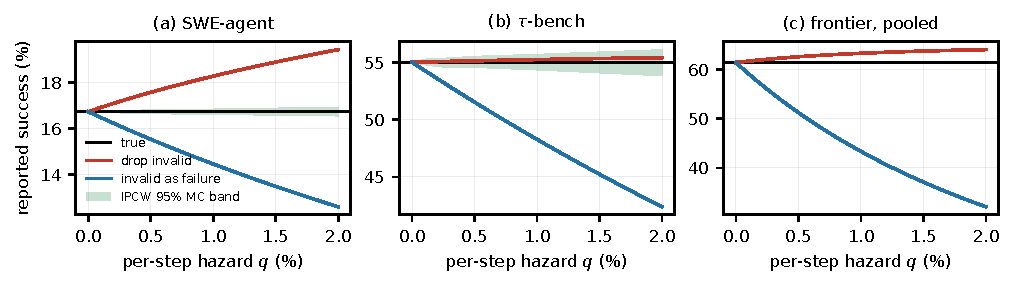
\includegraphics[width=\textwidth]{figures/fig_hazard.pdf}
\caption{Reported reliability against a declared per-step hazard. SWE-agent and
frontier successes survive better, so dropping invalid runs inflates
reliability; on $\tau$-bench the complete-case curve is almost flat. Scoring as
failure falls fastest on the frontier, whose runs are longest. Shaded: 95\%
Monte Carlo band of the Horvitz--Thompson estimator (200 replicates).}
\label{fig:hazard}
\end{figure}

\begin{table}[t]
\centering
\small
\setlength{\tabcolsep}{4pt}
\begin{tabular}{@{}lrrrrrrr@{}}
\toprule
corpus & $p$ & $\pb_1$ & $\pb_0$ & $\rho$ & $m$ (\%) & drop & fail \\
\midrule
SWE-agent & 16.73 & .864 & .777 & 1.113 & 20.9 & $+1.54$ & $-2.27$ \\
$\tau$-bench & 55.03 & .877 & .869 & 1.009 & 12.6 & $+0.23$ & $-6.75$ \\
Frontier, per model (range) & 19.8--76.8 & .45--.89 & .38--.86 & 0.90--1.39 & 12--57 &
$-2.7$ to $+7.9$ & $-38.4$ to $-2.8$ \\
\bottomrule
\end{tabular}
\caption{Three numbers at a declared $q=1\%$ and the resulting policy biases in
points. Proposition~\ref{prop:three} reproduces both biases exactly (error
$<10^{-15}$).}
\label{tab:three}
\end{table}

\paragraph{Three numbers explain the dissociation.} On SWE-agent the survival
ratio is well above one, so dropping inflates and scoring-as-failure deflates
reliability, a 6.8-point spread at $q=2\%$ (Figure~\ref{fig:hazard},
Table~\ref{tab:three}). On $\tau$-bench $\rho\approx1$, so dropping is nearly
safe while scoring-as-failure costs 12.6 points at $q=2\%$. On the frontier,
horizons are long (successes average 38 steps, failures 51), so a 1\% hazard
invalidates 12--57\% of a model's runs and scoring-as-failure costs up to 38.4
points (DeepSeek-V3.2 at high reasoning effort, whose successful runs average 83
steps).

\paragraph{The mean gap is not enough, and both policies can err downward.}
The first-order approximation $\log\rho\approx q(\bar H_0-\bar H_1)$ overstates
SWE-agent's $\log\rho$ by 26\% at $q=1\%$ and 48\% at $q=2\%$. Neither older
corpus satisfies stochastic dominance (Figure~\ref{fig:horizons}), yet $\rho>1$
at every $q\le5\%$. At model level, 5 of 29 $\tau$-bench models and 1 of 39
frontier models (Devstral 2512) have $\rho<1$; for these, dropping invalid runs also
understates reliability.

\begin{figure}[t]
\centering
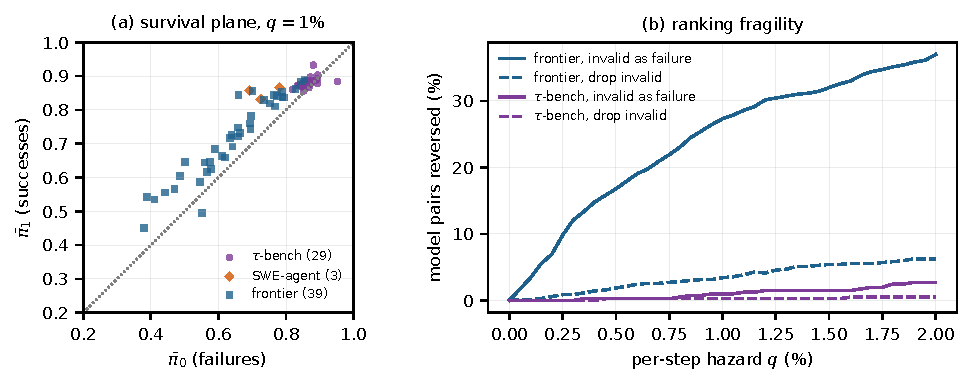
\includegraphics[width=\textwidth]{figures/fig_plane_fragility.pdf}
\caption{(a) Every model in the survival plane at $q=1\%$; above the diagonal,
dropping invalid runs overstates reliability. Frontier models spread far along
both axes because their horizons differ several-fold. (b) Share of model pairs
whose order reverses under a declared hazard.}
\label{fig:fragility}
\end{figure}

\paragraph{Frontier rankings are fragile.} Because frontier models are close in
score (median gap between adjacent models 1.0 point) and far apart in horizon,
their order is much more sensitive than that of older corpora
(Figure~\ref{fig:fragility}b). Under invalid-as-failure, the first reversal among
the 39 models occurs at $q=0.01\%$; at $q=0.1\%$, which invalidates 4.1\% of
runs on average, 24 of 741 pairs reverse; at $q=0.25\%$ (9.8\% invalid), 69; at
$q=1\%$, 192. Dropping invalid runs is gentler but not safe: 1, 6, and 24 pairs.
On $\tau$-bench the first reversal needs $q=0.32\%$.

\paragraph{Rerunning removes most, not all, of the bias.} On SWE-agent's 4{,}219
task$\times$model cells, rerunning until valid removes 70--72\% of the
complete-case bias at every hazard, leaving $+0.44$ points at $q=1\%$ at a cost
of 1.28 attempts per task (Proposition~\ref{prop:rerun}).

\paragraph{Cost, an unbounded metric.} Dropping invalid runs understates the
mean cost per task by 5--76\% across frontier models at $q=1\%$, because the
dropped runs are the long, expensive ones. No assumption-free bound exists for
cost; reports need an explicit model.

\section{Real Invalidity on Public Leaderboards}
\label{sec:real}

\begin{figure}[t]
\centering
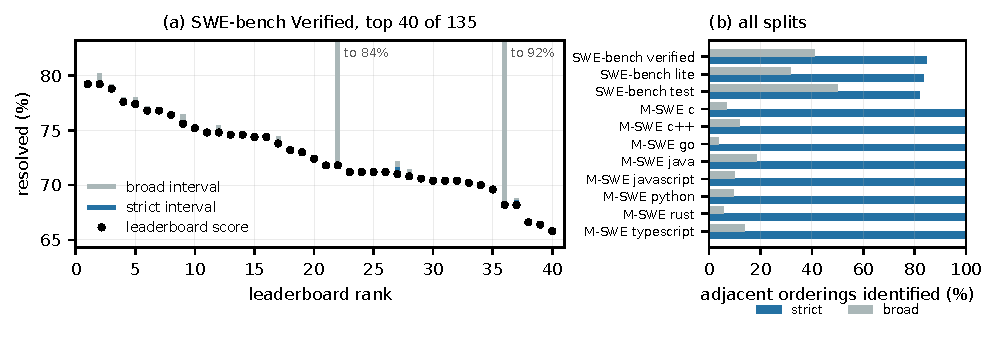
\includegraphics[width=\textwidth]{figures/fig_census.pdf}
\caption{Identified intervals for the top 40 of 135 SWE-bench Verified
submissions. Dots are leaderboard scores (resolved over 500), which are the lower
endpoints. Bars extend over evaluation-censored runs (strict) and additionally
over unattributable runs (broad).}
\label{fig:census}
\end{figure}

\paragraph{Census.} Across 243 SWE-bench submissions, invalidity is common and
leaderboard gaps are small (Figure~\ref{fig:census}). On Verified, 35\% of
submissions contain evaluation-censored runs (up to 18\% of a submission) and
70\% contain unattributable runs (median 0.4\%, up to 24.2\%); 15 submissions
have more than 5\% of runs in one of the two classes. The median gap between
adjacent submissions is 0.4 points, two tasks, and 61\% of adjacent gaps are at
most that. Consequently the data identify 89 of 105 adjacent orderings under the
strict reading and only 43 under the broad reading (Lite: 55 and 21 of 66;
Test: 18 and 11 of 22). Over all pairs the identified share is 98.8\% and
94.9\% on Verified: the leaderboard's coarse structure is sound, its fine
structure is not identified by the published evidence.

\begin{table}[t]
\centering
\small
\begin{tabular}{@{}lrrrrrr@{}}
\toprule
 & censored & leaderboard & bounds & complete & KM & rank \\
submission & runs & score & (strict) & case & weighted & LB $\to$ KM \\
\midrule
Qwen2.5-Coder-32B & 278 & 9.0 & [8.8, 64.4] & 19.8 & 10.3 & 38 $\to$ 38 \\
Gemini 3 Pro (high) & 11 & 70.6 & [70.6, 72.8] & 72.2 & 72.2 & 12 $\to$ 9 \\
gpt-oss-120b & 9 & 26.0 & [26.0, 27.8] & 26.5 & 26.3 & 36 $\to$ 36 \\
Gemini 3 Flash (high) & 3 & 75.8 & [75.8, 76.4] & 76.3 & 76.3 & 2 $\to$ 2 \\
\bottomrule
\end{tabular}
\caption{Real provider failures on the frontier leaderboard (resolved \%, 500
tasks each). Seven of 39 submissions have provider-censored runs; the four with
the most are shown. Ranks count models strictly ahead (ties share a rank).}
\label{tab:frontier}
\end{table}

\paragraph{Frontier provider failures.} Seven of 39 frontier submissions lost
runs to provider errors after the harness's retries, 305 runs in all, of which
304 are scored as unresolved (Table~\ref{tab:frontier}). Qwen2.5-Coder-32B lost 278 of
500 runs (56\%): its leaderboard score of 9.0\% is the lower end of an interval
that reaches 64.4\%. Complete-case reporting would give 19.8\%, but the failures
struck long runs, which rarely succeed, so Kaplan--Meier weighting with the
observed failure step gives 10.3\%, and the sensitivity analysis gives
9.2--13.9\% for $\gamma\in[1/4,4]$. The rank is unchanged either way. Gemini 3
Pro lost only 11 runs (2.2\%), but it sits in the densest part of the
leaderboard: weighting moves it from 12th (tied) to 9th, and it ranks 9th or
10th for every $\gamma\in[1/4,4]$, that is, even if its failed runs were four
times less likely to succeed than comparable completed runs.

\paragraph{Container failures in the SWE-agent corpus.} The corpus's
\texttt{early\_exit} status is set only when the container runtime raises during
a step \citep{sweagent2024code}. It marks 3{,}176 runs (4.0\%), none resolved.
The identified interval is $[16.73,20.70]\%$; complete-case gives 17.42\%;
model-stratified Kaplan--Meier gives 17.09\%; the doubly robust estimator, which
also uses each crashed run's logged prefix, gives 17.10\%; and $\gamma\in[1/4,4]$ gives 16.8--17.8\%. The corpus label is the lower
endpoint.

\section{Estimators in Practice}
\label{sec:estimators}

\paragraph{Weighting from observables.} Simulating failure times step by step
and estimating $G$ only from $(V_i,C_i)$, Kaplan--Meier weighting has bias at
most 0.015 points on SWE-agent and 0.008 on $\tau$-bench under constant hazards
up to 2\%, and at most 0.024 under a hazard that doubles after step 25, where a
constant-hazard fit is biased by $+0.33$ to $+0.67$ points. Estimated weights are
more efficient than true ones (standard deviation 0.25 against 0.37 points on
$\tau$-bench at $q=1\%$), as theory predicts \citep{robins1994estimation}.
Under a hard cap at 25 steps on SWE-agent, weighting collapses to the complete
case (23.04\% against a true 16.73\%) and only the bounds
$[15.05,49.73]\%$ remain valid.

\paragraph{Doubly robust estimation.} We fit $\mu$ by weighted logistic
regression on 16 prefix features and an intercept (elapsed steps; counts of edit, create, run,
and navigation actions; failed edits; observation errors; whether a clean run
followed the last edit; steps since the last edit; the model), with two-fold
cross-fitting by task and weights $\hat G(t-1)/\hat G(H_i)$ on completed runs.
The implementation satisfies the exactness identity of
Proposition~\ref{prop:dr} to machine precision. Prefixes are informative but far
from decisive: the in-sample AUC for eventual success (17 parameters on 2.1
million step rows) rises from 0.53 at step~1 to 0.71 at step~40
(Figure~\ref{fig:dr}b). Figure~\ref{fig:dr}a shows the three properties
the theory predicts. \emph{Robustness to the censoring model:} under the
step-dependent hazard, weighting with a constant-hazard fit is biased by $+0.68$
points, and adding the prefix model cuts the bias to $-0.03$. \emph{Robustness to
the outcome model:} with correct Kaplan--Meier weights, a deliberately wrong
constant $\mu=0.5$ leaves the estimator unbiased ($+0.01$). \emph{Efficiency:} at
$q=2\%$ the prefix model lowers the standard deviation from 0.133 to 0.084
points relative to constant-hazard weighting, and from 0.090 to 0.085 relative to
Kaplan--Meier weighting. On the real container failures the two agree
(17.10\%), which is consistent with those failures being unrelated to the prefix
features we model. The practical value of the prefix is
therefore insurance against a wrong censoring model, with modest efficiency
gains that should grow with better outcome models.

\begin{figure}[t]
\centering
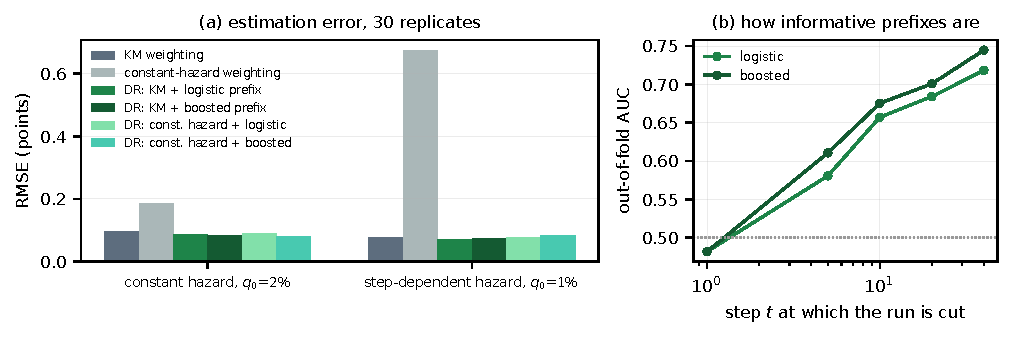
\includegraphics[width=\textwidth]{figures/fig_dr.pdf}
\caption{Estimation from partial trajectories on the SWE-agent corpus (50
replicates per scenario). (a) Root-mean-square error of five estimators under
constant and step-dependent declared hazards; the constant-hazard fit fails when
the hazard changes with step, and the doubly robust estimator repairs it. (b)
In-sample discrimination (AUC) of the prefix model by the step at which a run is
cut.}
\label{fig:dr}
\end{figure}

\section{A Minimum Validity Record}
\label{sec:practice}

Every estimator in this paper is computable from five fields per run:
(1) the task and agent; (2) the termination reason, classified by
Definition~\ref{def:validity}; (3) the step (and, if relevant, tokens and
wall-clock) at termination; (4) the outcome, if one was produced; and (5) the
number of attempts, if reruns were used. A report should then give the
initiated and valid run counts, invalid counts by class, the policy applied,
and the interval of Proposition~\ref{prop:bounds} next to the headline number.
None of the public artifacts we examined records all five fields in one place;
the frontier corpus comes closest, since its trajectories carry both exit status
and step count.

\section{Related Work}

\citet{zhao2026failure} anatomise coding-agent failure over complete
trajectories. \citet{ruan2026doomed} abort episodes predicted to fail; this
removes outcomes deliberately as a function of predicted failure, which is
outcome-dependent censoring outside our independent-failure model.
\citet{li2026early} study failure-aware observability but do not pose
infrastructure termination as a missing-outcome problem;
\citet{gonuguntla2026replay} shows static replay under a substituted model scores
a counterfactual world. \citet{wang2026interface} uses ``censoring'' for
interface-level output suppression, and \citet{raghu2026proper} extend proper
scoring rules to administratively censored trajectories, the closest work,
though it scores predictions rather than identifying an aggregate estimand.
Disclosure and validity work
\citep{kapoor2024agentsthatmatter,weidinger2025evalscience,zhu2026guardrails,chen2026judge,moghadasi2026disclose}
reports what happened; we study how missing outcomes change the estimand and
what the published evidence identifies. Our estimators are classical
\citep{horvitz1952generalization,kaplan1958nonparametric,manski1990nonparametric,robins1992recovery,robins1994estimation,bang2005doubly,scharfstein1999adjusting};
the contribution is their mapping onto agent evaluation, the three-number and
rerun results, the use of partial trajectories, and measurement on public
leaderboards.

\section{Limitations}

(1) The declared-hazard results are a sensitivity analysis; the real-censoring
results rest on exit statuses whose attribution we classify by
Definition~\ref{def:validity}, and some statuses are unattributable. (2)
Weighting assumes failure independent of the outcome given the observed prefix;
the $\gamma$ analysis bounds departures but does not remove them. (3) The census
reads published outcome lists; a submission's \texttt{no\_generation} may be the
agent's own choice, which is why we report strict and broad readings. (4) The
frontier corpus uses one scaffold on one benchmark, and two submissions required
label repair or exclusion. (5) Rankings use point estimates; we do not model
sampling uncertainty over tasks. (6) A controlled fault-injection study in a
live harness, with paired clean runs as ground truth, is the natural next test.

\section{Conclusion}

An invalid execution is not a failed one. On public leaderboards, runs lost to
providers, containers, and evaluation harnesses are scored as failures, which
reports the lower end of what the data identify; dropping them tilts the odds;
rerunning fixes only part. Because horizons differ several-fold across frontier
models, these choices reorder models at hazards far below what practitioners
routinely see. The remedy is cheap: record each run's termination reason and
step, report the identified interval, and estimate with weights, and with the
partial trajectory, when independence is defensible.

\bibliographystyle{plainnat}
\bibliography{references}

\appendix

\section{Proofs}
\label{app:proofs}

\paragraph{Proposition~\ref{prop:rerun}.} Attempts in cell $c$ are i.i.d.\ from
$F_c$, each valid with probability $G(H)$ independently, so the first valid
attempt has density $G(h)\,dF_c(y,h)/\E_c[G(H)]$ and success probability
$\E_c[Y\pi]/\E_c[\pi]=p_c+{\rm Cov}_c(Y,\pi)/\E_c[\pi]$. Averaging with weights
$w_c$ gives the first identity; the law of total covariance applied to
$p_{\rm cc}=\sum_cw_c\E_c[Y\pi]/\pb$ gives the second. The number of attempts is
geometric with mean $1/\E_c[\pi]$.

\paragraph{Proposition~\ref{prop:km}.} Under $T\perp(Y,H)$ the observed pairs
$(V_i,1-C_i)$ are a right-censored sample of $T$ with independent censoring by
$H$, so $\hat G$ is consistent for $G$ wherever the risk set is non-empty
\citep{kaplan1958nonparametric}. Since $\E[C_i\mid Y_i,H_i]=G(H_i)$, the
weighted numerator and denominator are consistent for $Np$ and $N$
\citep{satten2001kaplan}. Under a cap, every run with $H>K$ is invalidated at
$K+1$, so $\hat G(K+1)=0$ and valid runs all have weight $\hat G(H_i)^{-1}=1$.

\paragraph{Exactness in Proposition~\ref{prop:dr}.} Using
$1/G(t)-1/G(t-1)=\lambda(t)/G(t)$, a run invalidated at step $t_0$ contributes
$\sum_{t<t_0}(-\lambda(t))/G(t)+(1-\lambda(t_0))/G(t_0)=
(1-1/G(t_0-1))+1/G(t_0-1)=1$, and a completed run contributes
$1/G(H)+\sum_{t\le H}(-\lambda(t))/G(t)=1/G(H)+1-1/G(H)=1$. With
$\mu_t(x_{it})=Y_i$ each bracket therefore equals $Y_i$. Double robustness
follows from the standard argument \citep{tsiatis2006semiparametric}: the
augmentation has mean zero when $G$ is correct, and when $\mu$ is correct the
estimating function has mean zero for any $G$ \citep{bang2005doubly}.

\section{Additional Results}

\paragraph{Horizon distributions.} Figure~\ref{fig:horizons} shows the
outcome-conditional horizon distributions behind $\pb_1$ and $\pb_0$.

\begin{figure}[h]
\centering
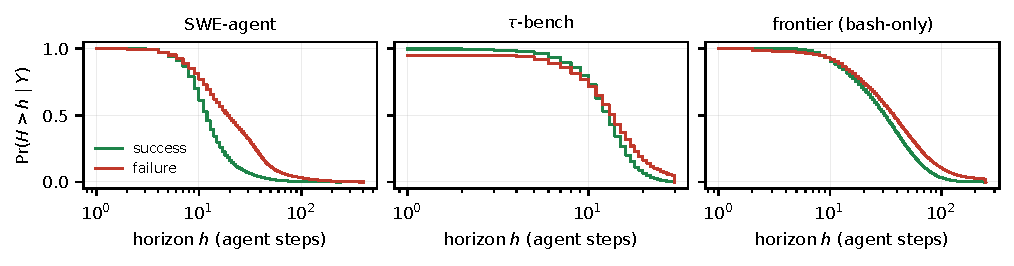
\includegraphics[width=\textwidth]{figures/fig_horizons.pdf}
\caption{Horizon survival $\Pr(H>h\mid Y)$ by outcome. On $\tau$-bench the
curves cross at short horizons, so stochastic dominance fails.}
\label{fig:horizons}
\end{figure}

\paragraph{Predeclared grids (symposium version).} SWE-agent, true $p=16.73\%$:
at $q=0.1/0.25/0.5/1/2\%$, $p_{\rm cc}=16.91/17.17/17.57/18.27/19.42$ and
$\E\hat p_{\rm fail}=16.48/16.11/15.53/14.46/12.60$. $\tau$-bench, true
$p=55.03\%$: $p_{\rm cc}=55.06/55.09/55.15/55.26/55.43$ and
$\E\hat p_{\rm fail}=54.31/53.26/51.54/48.28/42.39$. Horvitz--Thompson bias never
exceeds 0.005 (SWE-agent) or 0.017 points ($\tau$-bench).

\paragraph{Label repair and exclusion.} The bash-only submission for Gemini 3 Pro
(high) lists every run as unresolved in its per-instance file while its metadata
reports 69.6\%; its 500 public evaluation reports give 353 resolved (70.6\%),
which we use. The submission for Claude 3.7 Sonnet (mini-SWE-agent v0.0.0)
reports 52.8\% in metadata and 10.2\% in its per-instance file, and only 98 of
500 evaluation reports are public, so we exclude it.

\paragraph{Reproduction.} All inputs are public and no paid API is used.
\texttt{scripts/censoring/reproduce\_all.py} regenerates the symposium results;
the scripts in \texttt{scripts/extended/} then run in this order:
\begin{itemize}
\item \texttt{fetch\_swebench\_census.py}, \texttt{fetch\_bash\_only\_exits.py};
\item \texttt{repair\_labels.py}, \texttt{build\_prefix\_features.py};
\item \texttt{census\_leaderboard.py}, \texttt{frontier\_analysis.py},
\texttt{sensitivity.py}, \texttt{dr\_estimator.py};
\item \texttt{make\_extended\_figures.py}.
\end{itemize}

\end{document}
